\documentclass{standalone}
\usepackage{tikz}
\usetikzlibrary{patterns, positioning}
\usepackage[sfdefault]{ClearSans} %% option 'sfdefault' activates Clear Sans as the default text font
\usepackage[T1]{fontenc}

\begin{document}
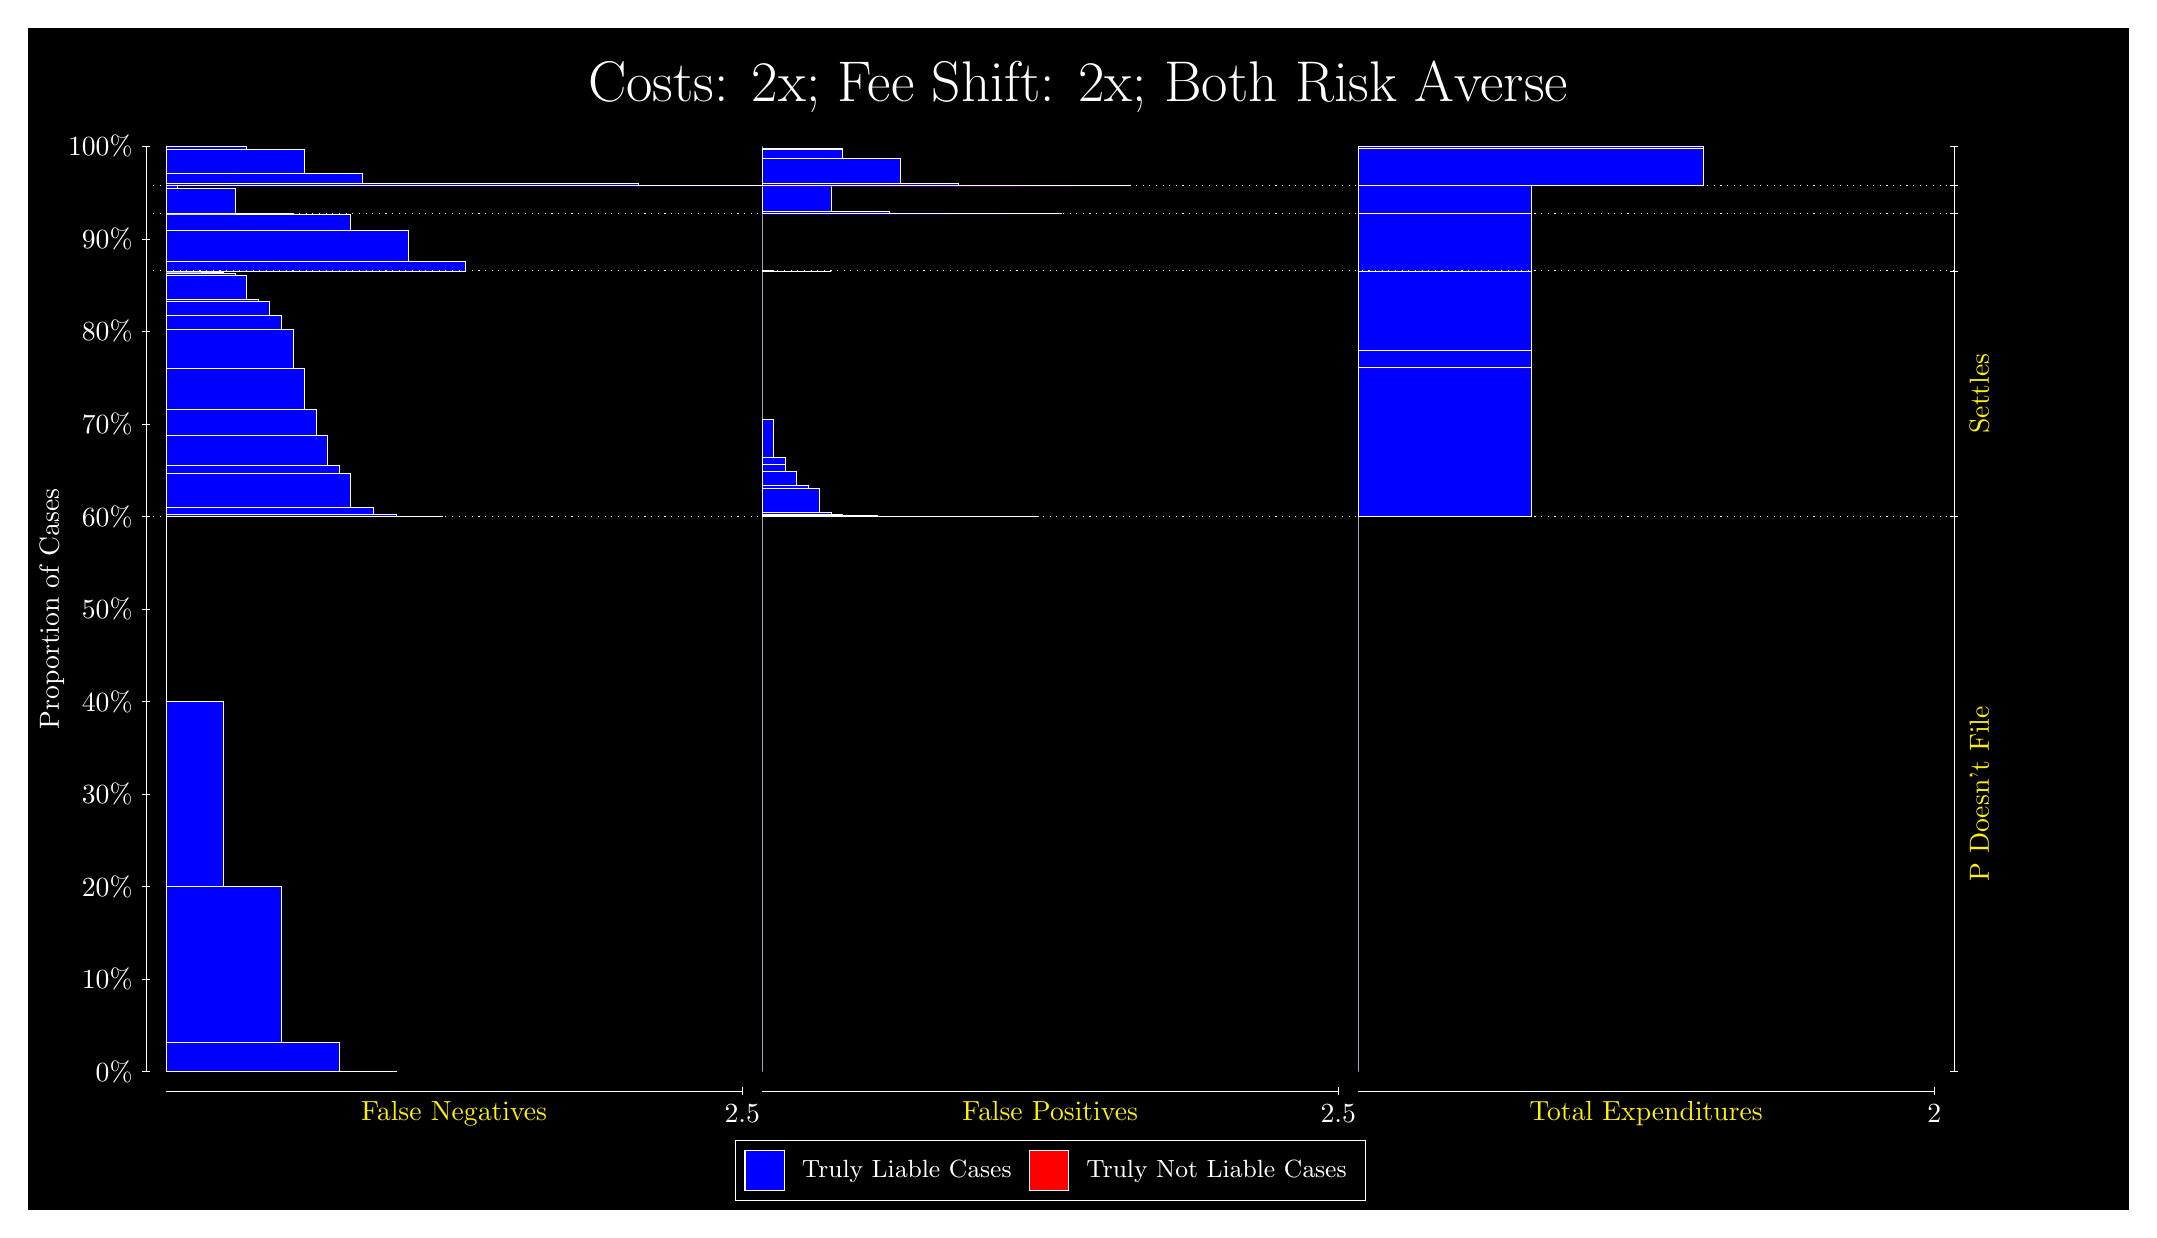
\begin{tikzpicture}
\draw[fill=black] (0,0) rectangle (26.667,15);
\draw[text=white] (0,13.5) rectangle (26.667,15) node[midway] {\huge Costs: 2x; Fee Shift: 2x; Both Risk Averse};
\draw[white, very thin] (1.5,1.75) -- (1.5,13.5);
\node[rotate=90, text=white, anchor=center] at (0.3, 7.625) {Proportion of Cases};
\draw[white, very thin] (1.45,1.75) -- (1.55,1.75);
\node[text=white, anchor=east] at (1.45, 1.75) {0\%};
\draw[white, very thin] (1.45,2.925) -- (1.55,2.925);
\node[text=white, anchor=east] at (1.45, 2.925) {10\%};
\draw[white, very thin] (1.45,4.1) -- (1.55,4.1);
\node[text=white, anchor=east] at (1.45, 4.1) {20\%};
\draw[white, very thin] (1.45,5.275) -- (1.55,5.275);
\node[text=white, anchor=east] at (1.45, 5.275) {30\%};
\draw[white, very thin] (1.45,6.45) -- (1.55,6.45);
\node[text=white, anchor=east] at (1.45, 6.45) {40\%};
\draw[white, very thin] (1.45,7.625) -- (1.55,7.625);
\node[text=white, anchor=east] at (1.45, 7.625) {50\%};
\draw[white, very thin] (1.45,8.8) -- (1.55,8.8);
\node[text=white, anchor=east] at (1.45, 8.8) {60\%};
\draw[white, very thin] (1.45,9.975) -- (1.55,9.975);
\node[text=white, anchor=east] at (1.45, 9.975) {70\%};
\draw[white, very thin] (1.45,11.15) -- (1.55,11.15);
\node[text=white, anchor=east] at (1.45, 11.15) {80\%};
\draw[white, very thin] (1.45,12.325) -- (1.55,12.325);
\node[text=white, anchor=east] at (1.45, 12.325) {90\%};
\draw[white, very thin] (1.45,13.5) -- (1.55,13.5);
\node[text=white, anchor=east] at (1.45, 13.5) {100\%};

\draw[white, very thin] (24.457,1.75) -- (24.457,13.5);
\draw[white, very thin] (24.407,1.75) -- (24.507,1.75);
\node[anchor=west] at (24.407, 1.75) {};
\draw[white, very thin] (24.407,8.8012) -- (24.507,8.8012);
\node[anchor=west] at (24.407, 8.8012) {};
\draw[white, very thin] (24.407,11.919) -- (24.507,11.919);
\node[anchor=west] at (24.407, 11.919) {};
\draw[white, very thin] (24.407,12.645) -- (24.507,12.645);
\node[anchor=west] at (24.407, 12.645) {};
\draw[white, very thin] (24.407,12.999) -- (24.507,12.999);
\node[anchor=west] at (24.407, 12.999) {};
\draw[white, very thin] (24.407,13.5) -- (24.507,13.5);
\node[anchor=west] at (24.407, 13.5) {};

\draw[white, very thin, fill=blue] (1.75,1.75) rectangle (4.6775,1.7538);
\draw[white, very thin, fill=blue] (1.75,1.7538) rectangle (3.9457,2.1271);
\draw[white, very thin, fill=blue] (1.75,2.1271) rectangle (3.2138,4.1043);
\draw[white, very thin, fill=blue] (1.75,4.1043) rectangle (2.4819,6.4512);
\draw[white, very thin, fill=red] (1.75,6.4512) rectangle (1.75,6.4512);
\draw[white, very thin, fill=blue] (1.75,6.4512) rectangle (1.75,8.8012);
\draw[white, very thin, fill=blue] (1.75,8.8012) rectangle (5.2631,8.802);
\draw[white, very thin, fill=blue] (1.75,8.802) rectangle (4.9703,8.8029);
\draw[white, very thin, fill=blue] (1.75,8.8029) rectangle (4.6775,8.8266);
\draw[white, very thin, fill=blue] (1.75,8.8266) rectangle (4.5312,8.8267);
\draw[white, very thin, fill=blue] (1.75,8.8267) rectangle (4.3848,8.8307);
\draw[white, very thin, fill=blue] (1.75,8.8307) rectangle (4.3848,8.916);
\draw[white, very thin, fill=blue] (1.75,8.916) rectangle (4.2384,8.9162);
\draw[white, very thin, fill=blue] (1.75,8.9162) rectangle (4.092,9.3514);
\draw[white, very thin, fill=blue] (1.75,9.3514) rectangle (3.9457,9.4534);
\draw[white, very thin, fill=blue] (1.75,9.4534) rectangle (3.7993,9.8308);
\draw[white, very thin, fill=blue] (1.75,9.8308) rectangle (3.6529,9.8316);
\draw[white, very thin, fill=blue] (1.75,9.8316) rectangle (3.6529,10.163);
\draw[white, very thin, fill=blue] (1.75,10.163) rectangle (3.5065,10.682);
\draw[white, very thin, fill=blue] (1.75,10.682) rectangle (3.5065,10.682);
\draw[white, very thin, fill=blue] (1.75,10.682) rectangle (3.3602,11.174);
\draw[white, very thin, fill=blue] (1.75,11.174) rectangle (3.2138,11.35);
\draw[white, very thin, fill=blue] (1.75,11.35) rectangle (3.0674,11.528);
\draw[white, very thin, fill=blue] (1.75,11.528) rectangle (3.0674,11.528);
\draw[white, very thin, fill=blue] (1.75,11.528) rectangle (2.921,11.528);
\draw[white, very thin, fill=blue] (1.75,11.528) rectangle (2.921,11.558);
\draw[white, very thin, fill=blue] (1.75,11.558) rectangle (2.921,11.559);
\draw[white, very thin, fill=blue] (1.75,11.559) rectangle (2.7746,11.868);
\draw[white, very thin, fill=blue] (1.75,11.868) rectangle (2.7746,11.868);
\draw[white, very thin, fill=blue] (1.75,11.868) rectangle (2.6283,11.892);
\draw[white, very thin, fill=blue] (1.75,11.892) rectangle (2.4819,11.903);
\draw[white, very thin, fill=blue] (1.75,11.903) rectangle (2.3355,11.908);
\draw[white, very thin, fill=blue] (1.75,11.908) rectangle (2.3355,11.908);
\draw[white, very thin, fill=blue] (1.75,11.908) rectangle (2.1891,11.908);
\draw[white, very thin, fill=blue] (1.75,11.908) rectangle (2.1891,11.908);
\draw[white, very thin, fill=blue] (1.75,11.908) rectangle (2.1891,11.908);
\draw[white, very thin, fill=blue] (1.75,11.908) rectangle (2.0428,11.919);
\draw[white, very thin, fill=blue] (1.75,11.919) rectangle (2.0428,11.919);
\draw[white, very thin, fill=blue] (1.75,11.919) rectangle (1.8964,11.919);
\draw[white, very thin, fill=red] (1.75,11.919) rectangle (1.75,11.919);
\draw[white, very thin, fill=blue] (1.75,11.919) rectangle (1.75,11.919);
\draw[white, very thin, fill=blue] (1.75,11.919) rectangle (5.5558,12.042);
\draw[white, very thin, fill=blue] (1.75,12.042) rectangle (4.8239,12.435);
\draw[white, very thin, fill=blue] (1.75,12.435) rectangle (4.092,12.642);
\draw[white, very thin, fill=blue] (1.75,12.642) rectangle (3.3602,12.645);
\draw[white, very thin, fill=blue] (1.75,12.645) rectangle (2.6283,12.645);
\draw[white, very thin, fill=red] (1.75,12.645) rectangle (1.75,12.645);
\draw[white, very thin, fill=blue] (1.75,12.645) rectangle (2.6283,12.97);
\draw[white, very thin, fill=blue] (1.75,12.97) rectangle (1.8964,12.999);
\draw[white, very thin, fill=red] (1.75,12.999) rectangle (1.75,12.999);
\draw[white, very thin, fill=blue] (1.75,12.999) rectangle (1.75,12.999);
\draw[white, very thin, fill=blue] (1.75,12.999) rectangle (9.9471,12.999);
\draw[white, very thin, fill=blue] (1.75,12.999) rectangle (9.2152,12.999);
\draw[white, very thin, fill=blue] (1.75,12.999) rectangle (8.4834,13.009);
\draw[white, very thin, fill=blue] (1.75,13.009) rectangle (7.7515,13.026);
\draw[white, very thin, fill=blue] (1.75,13.026) rectangle (7.0196,13.026);
\draw[white, very thin, fill=blue] (1.75,13.026) rectangle (6.2877,13.026);
\draw[white, very thin, fill=blue] (1.75,13.026) rectangle (5.7022,13.026);
\draw[white, very thin, fill=blue] (1.75,13.026) rectangle (5.5558,13.026);
\draw[white, very thin, fill=blue] (1.75,13.026) rectangle (4.9703,13.031);
\draw[white, very thin, fill=blue] (1.75,13.031) rectangle (4.2384,13.157);
\draw[white, very thin, fill=blue] (1.75,13.157) rectangle (3.5065,13.467);
\draw[white, very thin, fill=blue] (1.75,13.467) rectangle (2.7746,13.5);
\draw[white, very thin, fill=blue] (1.75,13.5) rectangle (2.0428,13.5);
\draw[white, very thin, fill=red] (1.75,13.5) rectangle (1.75,13.5);
\draw[white, very thin, fill=blue] (1.75,13.5) rectangle (1.75,13.5);
\draw[white, very thin, fill=red] (9.3189,1.75) rectangle (9.3189,1.75);
\draw[white, very thin, fill=blue] (9.3189,1.75) rectangle (9.3189,8.8012);
\draw[white, very thin, fill=red] (9.3189,8.8012) rectangle (12.832,8.8012);
\draw[white, very thin, fill=blue] (9.3189,8.8012) rectangle (12.832,8.8012);
\draw[white, very thin, fill=red] (9.3189,8.8012) rectangle (12.539,8.8012);
\draw[white, very thin, fill=blue] (9.3189,8.8012) rectangle (12.539,8.8012);
\draw[white, very thin, fill=red] (9.3189,8.8012) rectangle (12.246,8.8012);
\draw[white, very thin, fill=blue] (9.3189,8.8012) rectangle (12.246,8.8012);
\draw[white, very thin, fill=blue] (9.3189,8.8012) rectangle (12.1,8.8012);
\draw[white, very thin, fill=red] (9.3189,8.8012) rectangle (11.954,8.8012);
\draw[white, very thin, fill=blue] (9.3189,8.8012) rectangle (11.954,8.8012);
\draw[white, very thin, fill=blue] (9.3189,8.8012) rectangle (11.807,8.8012);
\draw[white, very thin, fill=red] (9.3189,8.8012) rectangle (11.661,8.8012);
\draw[white, very thin, fill=blue] (9.3189,8.8012) rectangle (11.661,8.8012);
\draw[white, very thin, fill=blue] (9.3189,8.8012) rectangle (11.515,8.8012);
\draw[white, very thin, fill=red] (9.3189,8.8012) rectangle (11.368,8.8012);
\draw[white, very thin, fill=blue] (9.3189,8.8012) rectangle (11.368,8.8012);
\draw[white, very thin, fill=blue] (9.3189,8.8012) rectangle (11.222,8.8012);
\draw[white, very thin, fill=blue] (9.3189,8.8012) rectangle (11.075,8.8012);
\draw[white, very thin, fill=red] (9.3189,8.8012) rectangle (11.075,8.8012);
\draw[white, very thin, fill=blue] (9.3189,8.8012) rectangle (11.075,8.8012);
\draw[white, very thin, fill=blue] (9.3189,8.8012) rectangle (10.929,8.8012);
\draw[white, very thin, fill=red] (9.3189,8.8012) rectangle (10.783,8.8012);
\draw[white, very thin, fill=blue] (9.3189,8.8012) rectangle (10.783,8.8116);
\draw[white, very thin, fill=blue] (9.3189,8.8116) rectangle (10.636,8.8117);
\draw[white, very thin, fill=red] (9.3189,8.8117) rectangle (10.49,8.8117);
\draw[white, very thin, fill=blue] (9.3189,8.8117) rectangle (10.49,8.8117);
\draw[white, very thin, fill=blue] (9.3189,8.8117) rectangle (10.49,8.8163);
\draw[white, very thin, fill=blue] (9.3189,8.8163) rectangle (10.344,8.8275);
\draw[white, very thin, fill=blue] (9.3189,8.8275) rectangle (10.344,8.8277);
\draw[white, very thin, fill=blue] (9.3189,8.8277) rectangle (10.197,8.8518);
\draw[white, very thin, fill=blue] (9.3189,8.8518) rectangle (10.051,9.161);
\draw[white, very thin, fill=blue] (9.3189,9.161) rectangle (9.9044,9.1917);
\draw[white, very thin, fill=blue] (9.3189,9.1917) rectangle (9.758,9.1917);
\draw[white, very thin, fill=blue] (9.3189,9.1917) rectangle (9.758,9.3693);
\draw[white, very thin, fill=blue] (9.3189,9.3693) rectangle (9.6116,9.4578);
\draw[white, very thin, fill=blue] (9.3189,9.4578) rectangle (9.6116,9.5453);
\draw[white, very thin, fill=blue] (9.3189,9.5453) rectangle (9.4652,10.038);
\draw[white, very thin, fill=blue] (9.3189,10.038) rectangle (9.3189,11.919);
\draw[white, very thin, fill=red] (9.3189,11.919) rectangle (10.197,11.919);
\draw[white, very thin, fill=blue] (9.3189,11.919) rectangle (10.197,11.919);
\draw[white, very thin, fill=blue] (9.3189,11.919) rectangle (9.4652,11.921);
\draw[white, very thin, fill=blue] (9.3189,11.921) rectangle (9.3189,12.645);
\draw[white, very thin, fill=red] (9.3189,12.645) rectangle (13.125,12.645);
\draw[white, very thin, fill=blue] (9.3189,12.645) rectangle (13.125,12.645);
\draw[white, very thin, fill=blue] (9.3189,12.645) rectangle (12.393,12.645);
\draw[white, very thin, fill=blue] (9.3189,12.645) rectangle (11.661,12.645);
\draw[white, very thin, fill=blue] (9.3189,12.645) rectangle (10.929,12.674);
\draw[white, very thin, fill=blue] (9.3189,12.674) rectangle (10.197,12.999);
\draw[white, very thin, fill=red] (9.3189,12.999) rectangle (14.003,12.999);
\draw[white, very thin, fill=blue] (9.3189,12.999) rectangle (14.003,12.999);
\draw[white, very thin, fill=red] (9.3189,12.999) rectangle (13.271,12.999);
\draw[white, very thin, fill=blue] (9.3189,12.999) rectangle (13.271,12.999);
\draw[white, very thin, fill=red] (9.3189,12.999) rectangle (12.539,12.999);
\draw[white, very thin, fill=blue] (9.3189,12.999) rectangle (12.539,12.999);
\draw[white, very thin, fill=blue] (9.3189,12.999) rectangle (11.807,13.032);
\draw[white, very thin, fill=red] (9.3189,13.032) rectangle (11.807,13.032);
\draw[white, very thin, fill=blue] (9.3189,13.032) rectangle (11.807,13.032);
\draw[white, very thin, fill=blue] (9.3189,13.032) rectangle (11.075,13.342);
\draw[white, very thin, fill=blue] (9.3189,13.342) rectangle (11.075,13.342);
\draw[white, very thin, fill=blue] (9.3189,13.342) rectangle (10.344,13.467);
\draw[white, very thin, fill=blue] (9.3189,13.467) rectangle (10.344,13.469);
\draw[white, very thin, fill=blue] (9.3189,13.469) rectangle (9.6116,13.473);
\draw[white, very thin, fill=blue] (9.3189,13.473) rectangle (9.6116,13.473);
\draw[white, very thin, fill=red] (9.3189,13.473) rectangle (9.3189,13.473);
\draw[white, very thin, fill=blue] (9.3189,13.473) rectangle (9.3189,13.5);
\draw[white, very thin, fill=red] (16.888,1.75) rectangle (16.888,1.75);
\draw[white, very thin, fill=blue] (16.888,1.75) rectangle (16.888,8.8012);
\draw[white, very thin, fill=red] (16.888,8.8012) rectangle (19.083,8.8012);
\draw[white, very thin, fill=blue] (16.888,8.8012) rectangle (19.083,10.691);
\draw[white, very thin, fill=red] (16.888,10.691) rectangle (19.083,10.691);
\draw[white, very thin, fill=blue] (16.888,10.691) rectangle (19.083,10.912);
\draw[white, very thin, fill=red] (16.888,10.912) rectangle (19.083,10.912);
\draw[white, very thin, fill=blue] (16.888,10.912) rectangle (19.083,11.919);
\draw[white, very thin, fill=red] (16.888,11.919) rectangle (19.083,11.919);
\draw[white, very thin, fill=blue] (16.888,11.919) rectangle (19.083,12.645);
\draw[white, very thin, fill=red] (16.888,12.645) rectangle (19.083,12.645);
\draw[white, very thin, fill=blue] (16.888,12.645) rectangle (19.083,12.999);
\draw[white, very thin, fill=red] (16.888,12.999) rectangle (21.279,12.999);
\draw[white, very thin, fill=blue] (16.888,12.999) rectangle (21.279,13.471);
\draw[white, very thin, fill=red] (16.888,13.471) rectangle (21.279,13.471);
\draw[white, very thin, fill=blue] (16.888,13.471) rectangle (21.279,13.473);
\draw[white, very thin, fill=red] (16.888,13.473) rectangle (21.279,13.473);
\draw[white, very thin, fill=blue] (16.888,13.473) rectangle (21.279,13.5);
\draw[white, dotted] (1.5,8.8012) -- (24.457,8.8012);
\draw[white, dotted] (1.5,11.919) -- (24.457,11.919);
\draw[white, dotted] (1.5,12.645) -- (24.457,12.645);
\draw[white, dotted] (1.5,12.999) -- (24.457,12.999);
\draw[white, very thin] (1.75,1.5) -- (9.0689,1.5);
\node[text=yellow, anchor=north] at (5.4094, 1.5) {False Negatives};
\draw[white, very thin] (9.0689,1.45) -- (9.0689,1.55);
\node[text=white, anchor=north] at (9.0689, 1.45) {2.5};

\draw[white, very thin] (9.3189,1.5) -- (16.638,1.5);
\node[text=yellow, anchor=north] at (12.978, 1.5) {False Positives};
\draw[white, very thin] (16.638,1.45) -- (16.638,1.55);
\node[text=white, anchor=north] at (16.638, 1.45) {2.5};

\draw[white, very thin] (16.888,1.5) -- (24.207,1.5);
\node[text=yellow, anchor=north] at (20.547, 1.5) {Total Expenditures};
\draw[white, very thin] (24.207,1.45) -- (24.207,1.55);
\node[text=white, anchor=north] at (24.207, 1.45) {2};

\node[text=yellow, centered, rotate=90] at (24.777, 5.2756) {P Doesn't File};
\node[text=yellow, centered, rotate=90] at (24.777, 10.36) {Settles};




\draw (12.978300999999998,1.5) node[draw=none] (baseCoordinate) {};
\begin{scope}[align=center]
        \matrix[scale=0.5, draw=white, below=0.5cm of baseCoordinate, nodes={draw}, column sep=0.1cm]{
            \node[rectangle, draw, minimum width=0.5cm, minimum height=0.5cm, fill=blue] {}; &
            \node[draw=none, font=\small, text=white] (B) {Truly Liable Cases}; &
            \node[rectangle, draw, minimum width=0.5cm, minimum height=0.5cm, fill=red] {}; &
            \node[draw=none, font=\small, text=white] (B) {Truly Not Liable Cases}; \\
            };
\end{scope}

\end{tikzpicture}
\end{document}